% #############################################################################
% This is Appendix Model Integrations
% !TEX root = main.tex
% #############################################################################
\chapter{Model Integrations}
\label{chap:app003}

Lorem ipsum dolor sit amet, consectetur adipiscing elit, sed do eiusmod tempor incididunt ut labore et dolore magna aliqua. Ut enim ad minim veniam, quis nostrud exercitation ullamco laboris nisi ut aliquip ex ea commodo consequat. Duis aute irure dolor in reprehenderit in voluptate velit esse cillum dolore eu fugiat nulla pariatur. Excepteur sint occaecat cupidatat non proident, sunt in culpa qui officia deserunt mollit anim id est laborum.

Sed ut perspiciatis unde omnis iste natus error sit voluptatem accusantium doloremque laudantium, totam rem aperiam, eaque ipsa quae ab illo inventore veritatis et quasi architecto beatae vitae dicta sunt explicabo. Nemo enim ipsam voluptatem quia voluptas sit aspernatur aut odit aut fugit, sed quia consequuntur magni dolores eos qui ratione voluptatem sequi nesciunt. Neque porro quisquam est, qui dolorem ipsum quia dolor sit amet, consectetur, adipisci velit, sed quia non numquam eius modi tempora incidunt ut labore et dolore magnam aliquam quaerat voluptatem. Ut enim ad minima veniam, quis nostrum exercitationem ullam corporis suscipit laboriosam, nisi ut aliquid ex ea commodi consequatur? Quis autem vel eum iure reprehenderit qui in ea voluptate velit esse quam nihil molestiae consequatur, vel illum qui dolorem eum fugiat quo voluptas nulla pariatur?

\section{Neural Network Integration}
\label{sec:app003001}

In this section, we provide additional details concerning the use of the DenseNet that is integrated in our UI.
Concretely, we provide additional details concerning:
(i) the dataset;
(ii) data pre-processing;
(iii) evaluation strategy;
(iv) learning methodology;
(v) transfer learning; and
(vi) additional description of the system.

\subsection{Comparison with Existing Methodologies}
\label{sec:app003001001}

In terms of model comparison with already existing methods, the literature shows improvements of the DenseNet model concerning mean sensitivity and specificity by surpassing, as an example, the EfficientNet model~\cite{jpm10040211}.
For instance, the authors report the Mean AUC for detecting breast cancer was 0.952~\textpm~0.005 by a DenseNet model and 0.954~\textpm~0.020 by an EfficientNet model.
Moreover, the authors further report the mean sensitivity and specificity from a DenseNet model, of 87\% and 88\%, respectively, surpassed the mean values, of 81\% and 82\%, respectively, obtained in their meta-analysis.
Hence, the literature has demonstrated the DenseNet model efficiency~\cite{8633197, Hai2019, Zhong_2020}.

\subsection{Dataset Size}
\label{sec:app003001002}

In this paper, we used a total of 338 cases and acquired in the Hospital Fernando Fonseca.
From this set of cases, 289 were classified by the head of radiology.
Each patient has several images concerning four  X-ray mammography (two in CC and two MLO views), one ultrasound image, and roughly 5 images in MRI.
In the MRI volumes, we take several image slices per patient, where the lesion is present (recall point 5) in the previous question).
This provides us roughly 2890 images ({\it i.e.}, 289~\texttimes~(4 + 1 + 5)), that is used to train/test the AI agent (DenseNet).

\subsection{Data Pre-Processing}
\label{sec:app003001003}

Traditional image processing and deep learning techniques require extensive pre-processing~\cite{Zhong_2020}.
As a matter of fact, it is known that a cleaning dataset is welcome when training a deep neural network~\cite{RIASATIAN2021102032}.
In our study this stage is of the utmost importance, since the MG, US and MR images contain quite different intensities and the images are of different sizes.
Thus, before introducing the images to the DenseNet, we pre-process the data.
Specifically, we perform a data normalization, so that the images have the same intensity, regardless of the modality.

All the images are resized to 224x224 pixels.
Also, the images are normalized by subtracting its mean and dividing by its standard deviation.
The above size is used since the DenseNet is prepared to receive the input with this format.

\subsection{DenseNet Steps}
\label{sec:app003001004}

\hfill

\noindent
The DenseNet steps are as follows:

\hfill

\begin{enumerate}
\item The DenseNet is pre-trained with the ImageNet model that contains roughly 1.2 millions images. This gives generalization capabilities to new datasets.
\item Next, we remove the last layer of the DenseNet (that contains a large number of classes, about 1000 classes or end-nodes) and replace it by a fully connected layer containing now three nodes. Each node of the network corresponds to one of the following classes: (i) low severity (Class 1: BIRADS <= 1 ), (ii) medium severity  (Class 2:  1 < BIRADS <= 3) and (iii) high severity (Class 3: BIRADS > 3). Thus, we have a DenseNet with three nodes in the last layer.
\hfill
\item Now, the pre-trained DenseNet goes through a process of fine-tuning in our breast dataset. The dataset comprises 1125 training images ({\it i.e.}, MG in both CC and MLO views, US, and MRI). Notice that here, we have 338 cases or patients (Section~\ref{sec:procedure}). The larger number of training images, when compared to the number of patients, stems from the fact that one patient may have more than one image.
\hfill
\item We split the above dataset in the following way: 80\% for training and the remaining 20\% for testing. In this partition, we guarantee that each set (training and test) are properly balanced, that is, each set contains samples that belong to all classes (recall that there are three classes as mentioned in Section~\ref{sec:procedure}, see also point 1) and all modalities ({\it i.e.}, MG, US, and MRI). Therefore, the experiments take into consideration the multimodality.
\hfill
\item The pre-training follows a supervised learning strategy. Specifically, during the training we provide the image, as well as the corresponding label, that is, the classification in one of the three classes for the image. This classification ({\it i.e.}, ground-truth) is provided by a set of eight radiologists (Section~\ref{sec:methods}). Say that this training stage gives to the DenseNet the ability to establish associations between the morphology of the lesion (image) and its severity (classification label).
\hfill
\item Finally, we use the held-out test set to measure the performance of the DenseNet. An accuracy of 98.2\% was obtained in this test set.
\hfill
\item As a final note, we should mention that the three patients (as mentioned in Section~\ref{sec:participants}) are obtained from the test set as mentioned above (see point 4). 
From the above the number of test samples is high, however, only three samples are taken  for the experiments purpose. Thus, the training and testing phases take into account a large number of samples.
\end{enumerate}

\section{Training and Evaluation of the DenseNet}
\label{sec:app003002}

The evaluation mechanism for the DenseNet follows a two stage process, involving a training and testing stages.
To accomplish this, we partition the dataset (see Section~\ref{sec:sec010002}) to form the training and testing subsets in the following manner:
80\% of the samples are used for training and the remaining 20\% for testing.
In this partition, we guarantee that each set (training and test) is properly balanced.
That is, each set contains samples that belong to all five and in all modalities ({\it i.e.}, MG, US and MRI) - this is to guarantee  the multimodality.

\vspace{1mm}

\noindent
{\it Training}:
The training follows a supervised learning strategy.
Specifically, during the training we provide the image, as well as the corresponding label, that is, the classification BI-RADS score.
This classification ({\it i.e.}, ground truth) is provided by the head of radiology of the HFF institution.
This allows the DenseNet the ability to establish associations between the morphology of the lesion (image) and its severity (classification label).

\vspace{1mm}

\noindent
{\it Testing}:
During the test phase, we used a hold-out test set that aimed to measure  the performance of the DenseNet.
An accuracy of 94.81\% was obtained in this test set. 
Notice that the three patients (as mentioned in Sec 4.4) are obtained from this hold-out test set.

\vspace{2mm}

\noindent
{\it Remark}: 
Another possibility for the DenseNet training is to resort to unsupervised learning  methods. However, this class of approaches is more challenging, since only the images are fed into the network without the help of having the classification labels ({\it i.e.}, without BI-RADS classification in training).
This deserves our attention in a future work.

\section{Transfer Learning}
\label{sec:app003003}

As a final remark, we should stress that although the  number of samples is relatively small (3000 as mentioned in Section~\ref{sec:sec010002}), we may argue that this could be not enough, since a robust training DNNs usually requires large amounts of annotated samples (order of 100Ks) to avoid overfitting to the training data given the large model capacity.
This issue can be handled with the so-called ``Transfer Learning'' (TL).
Basically, the TL process retrains (in a process called fine-tuning) publicly available models (pre-trained with large datasets) using smaller datasets.

To initialize the weights of the network, the DenseNet model was pre-trained on the ImageNet dataset~\cite{deng2009imagenet} with more than 1.2 million images, which yields fast convergence for deep architectures~\cite{8515234}.
We used the DenseNet model by following two particular literature works for the classification of mammograms~\cite{10.1007/978-3-030-88163-4_16, 10.1007/978-3-030-47679-3_23}.

It has been demonstrated that this TL approach is possible to be applied in the medical image field, even if the datasets used in this pre-training stage are completely different from the medical images - in this case - different from breast images~\cite{10.1007/978-3-319-24574-4_78, 8032490}.
This is precisely what we did here.
Concretely, we used a pre-trained that provides the DNN more regularization and generalization capabilities to new datasets.
In the experiments, the DenseNet was pre-trained with the  ImageNet model that contains millions of images from 1000 classes (Section~\ref{sec:sec004005}).
The only adaptation required  to adapt the DenseNet, is to change the last layer from 1000 nodes (or classes) to the number of five classes in our problem.

\section{DenseNet Final Remarks}
\label{sec:app003004}

The DenseNet is a complex model.
This means that the model can handle heterogeneous types of the input.
Thus, given the relatively small number of training samples, it is advantageous to join all the modalities.

\vspace{2mm}

\noindent
In the experiments, we have compared two situations:

\vspace{2mm}

\begin{enumerate}
\item Joining all the modalities to a single DenseNet; and
\item Using three different DenseNet, each network for each image modality type (MG, US and MRI).
\end{enumerate}

\vspace{2mm}

The best results were achieved for situation (1), and this was adopted for our UI.

\section{Additional Description of the System}
\label{sec:app003005}

\vspace{2mm}

\noindent
Now we detail a little better the description of the system, as follows:

\begin{enumerate}
\item Each of the 289 patients was classified by the head of radiology of the Medical Imaging Department at the HFF institution. This classification corresponds to assigning a BI-RADS value for each modality image of the exam;
\item We trained our DenseNet across the BI-RADS, (we already detailed how the  training/test of the DenseNet is accomplished);
\item After the training, we have the test phase. Here the new (unseen) images are presented to the DenseNet, and a BI-RADS classification is provided to that test sample; and
\item To evaluate the accuracy of the system, the precision and recall are computed.
\end{enumerate}

\vspace{2mm}

\noindent
The following link is available that illustrates eases the description of the proposed system, as well as its workflow:

\vspace{2mm}

\noindent
\href{https://youtu.be/k2vBpbKqJqQ}{youtu.be/k2vBpbKqJqQ}


%%%%%%%%%%%%%%%%%%%%%%%%%%%%%%%%%%%%%%%%%%%%%%%%%%%
\begin{figure*}[htbp]
\centering
\captionsetup{justification=centering}
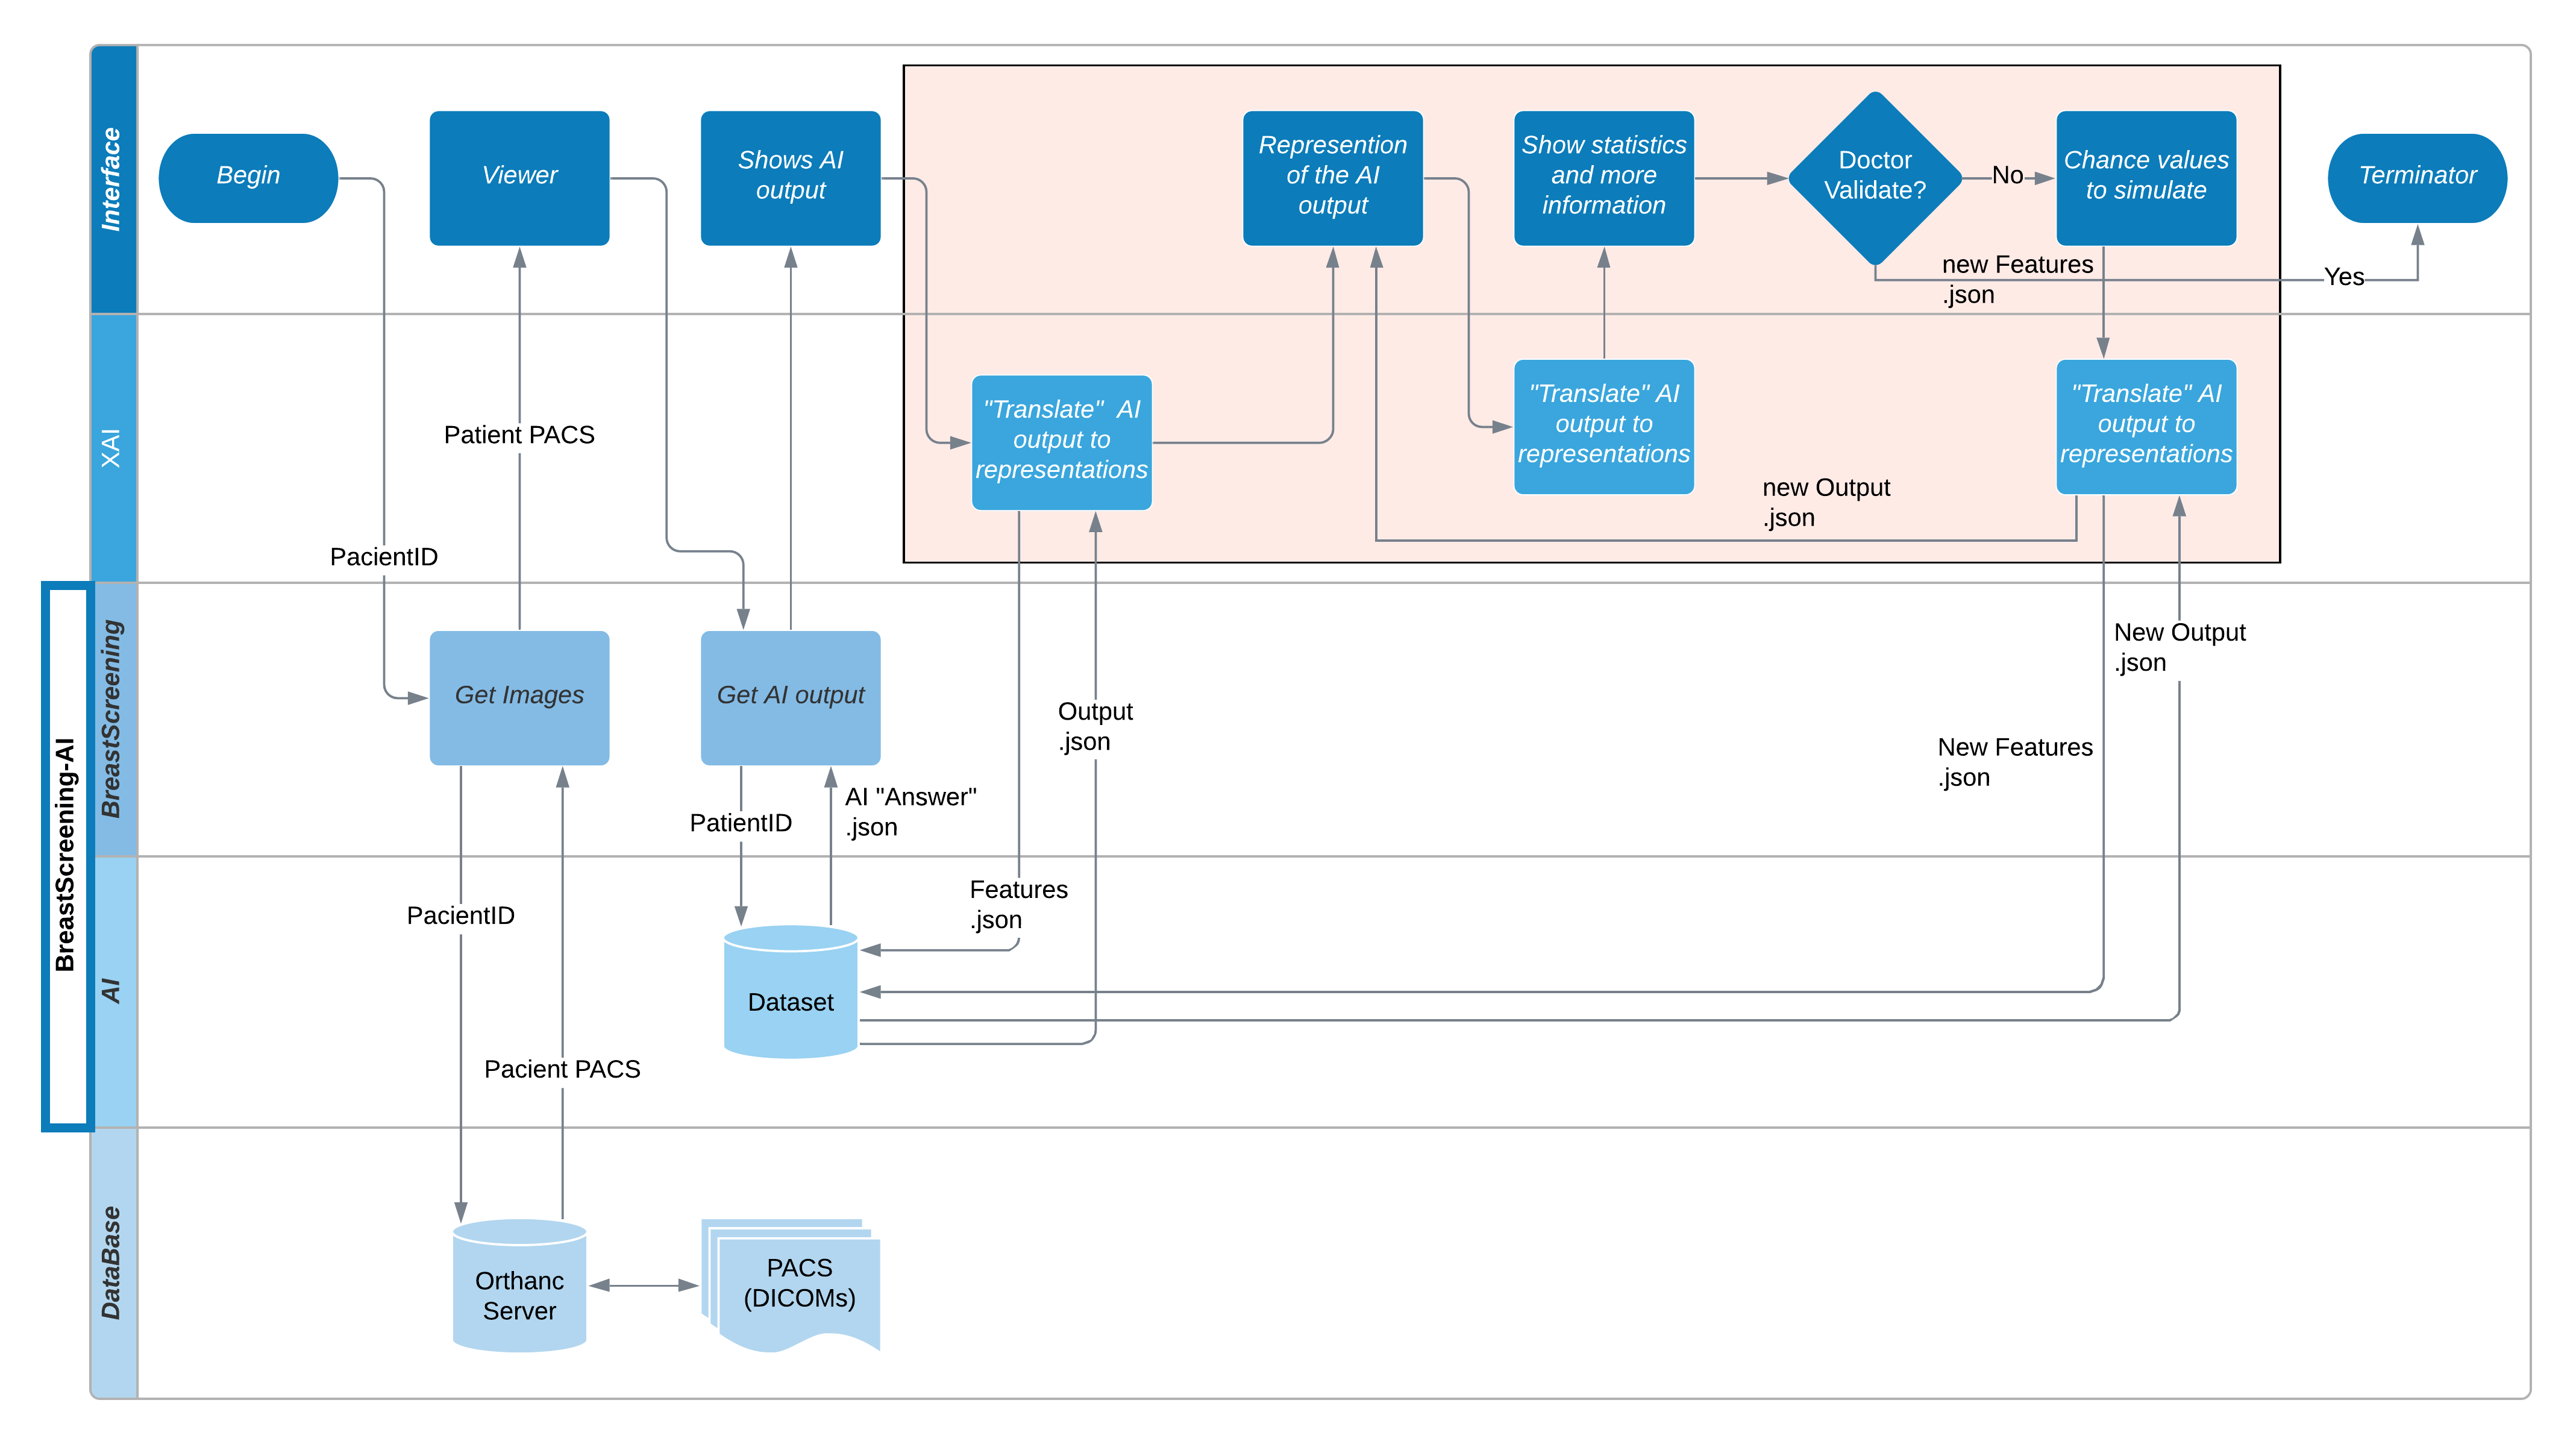
\includegraphics[width=0.925\textwidth]{fig072}
\caption{Architecture and functionalities diagram~\cite{nadia2020xai} of the typical use cases. These use cases are presented with the order of actions for the interrogated AI system.}
\label{fig:fig072}
\end{figure*}
%%%%%%%%%%%%%%%%%%%%%%%%%%%%%%%%%%%%%%%%%%%%%%%%%%%

\section{Separate vs. All Modalities}
\label{sec:app003006}

As shown in Table~\ref{tab:tab006}, the performance in the multimodal scenario is significantly higher than in the unimodal case.
This is a consequence of substantially increasing the training dataset when using all imaging modalities, which means the model is trained with a much larger number of images and with higher variability.
This increase in data helps regularize the DenseNet model, preventing over-fitting and improving its generalization capabilities.
In the unimodal case, the lack of a large training dataset resulted in severe over-fitting issues, despite our efforts to mitigate this through:
(i) data augmentation strategies, where each image is randomly modified in each batch using common transformations, such as small rotations, flipping, and translations; and
(ii) other regularization strategies like dropout and L2 (weight decay).

As a final remark, we stress that the network architecture receives 2D images.
Since the DCE-MRI are volumes, we extract some of the slices that contain the lesion.
All the above issues led the network to obtain significantly better results in the multimodal scenario, as demonstrated in Table~\ref{tab:tab016}.

\section{System Diagram}
\label{sec:app003007}

Concerning the system diagram~\cite{mourao2020architecture} of the BreastScreening-AI framework (Figure~\ref{fig:fig072}), the first action is to request the patients (Section~\ref{sec:sec004003}) stored on the Orthanc server~\cite{Jodogne2018}.
Next, the assistant will show the AI outputs~\cite{10.13140/RG.2.2.12519.16803, nadia2020xai}.
Finally, clinicians can decide by accepting or rejecting the AI suggestion.

As stated before (Section~\ref{sec:sec004}), our interface (Figure~\ref{fig:fig002}) has three main button functionalities ({\it i.e.}, 6.1. Accept; 6.2. Explain; and 6.3. Reject).
Each button of our interface is generating different triggers~\cite{10.1145/3436954} on the framework (Figure~\ref{fig:fig072}).
Hence, three triggers are important to denote.

%%%%%%%%%%%%%%%%%%%%%%%%%%%%%%%%%%%%%%%%%%%%%%%%%%%
\begin{table}[htpb]
\centering
\resizebox{\linewidth}{!}{%
\begin{tabular}{|c|cccc|c|}
\hline
Strategy   & \multicolumn{4}{c|}{Unimodal}                                                                  & \multirow{2}{*}{Multimodal} \\ \cline{1-5}
Modalities & \multicolumn{1}{c|}{CC-MG} & \multicolumn{1}{c|}{MLO-MG} & \multicolumn{1}{c|}{US}   & DCE-MRI &                             \\ \hline
Accuracy   & \multicolumn{1}{c|}{0.73}  & \multicolumn{1}{c|}{0.68}   & \multicolumn{1}{c|}{0.65} & 0.667   & 0.9481                      \\ \hline
\end{tabular}%
}
\caption{Evaluation results of the AI-Only for the unimodal tests with the DenseNet-121 model. Compared Models as unimodal training: Cranio-Caudal MG (CC-MG); Medio-Lateral Oblique MG (MLO-MG); UltraSound (US); and Dynamic Contrast-Enhanced MRI (DCE-MRI). Finaly, the multimodal training stands for CC-MG, MLO-MG, US, and DCE-MRI all modalities together.}
\label{tab:tab006}
\end{table}
%%%%%%%%%%%%%%%%%%%%%%%%%%%%%%%%%%%%%%%%%%%%%%%%%%%

The first trigger is made by clinicians when pressing the accept button, where a JSON file is generated to provide success information to the model~\cite{10.13140/rg.2.2.14792.55049}.
The second trigger represents the AI model explanations.
Clinicians press the explain button, in order of having more reliable information concerning what regions were considered by the model and how severe are these lesions to the model.
Finally, the third trigger happens when clinicians are rejecting the AI result.
At this point, clinicians must provide the new BI-RADS so that we can further retrain the AI model.
To this end, the framework will generate a JSON file with the new rejected BI-RADS values provided by clinicians.